\documentclass[a4paper,11pt,notitlepage]{article}
\usepackage{amsmath}
\usepackage{amsfonts}
\usepackage{amssymb}
\usepackage[UTF8]{ctex}
\usepackage{graphicx}
\usepackage{color}
\usepackage{changepage}
\usepackage{enumitem}
\usepackage{subfigure}
\usepackage{float}
\usepackage[backend=biber]{biblatex}

\usepackage{titlesec}
\titleformat{\section}{\bfseries\Large}{$\S$\,\thesection}{1em}{}
\titleformat{\subsection}{\bfseries\large}{\Roman{subsection}}{1em}{}
\titleformat{\subsubsection}{\bfseries\normalsize}{\roman{subsubsection}}{1em}{}
\titlespacing*{\subsection}{2em}{2pt}{2pt}
\titlespacing*{\subsubsection}{3em}{2pt}{2pt}
\title{\vspace{-1.5cm} \textbf{\huge{数值分析第12章上机}}\vspace{-1em}}
\author{By 211870125 陈睿硕}
\date{}

\usepackage{geometry}
\geometry{left=2cm,right=2cm,top=2cm,bottom=2cm}

\usepackage{fancyhdr}
\pagestyle{fancy}
\fancyhf{}
\fancyhead[L]{Chapter 12}
\fancyhead[R]{\thepage}
\setlength{\headheight}{14pt}

\usepackage{listings}  % 引入 listings 包
\lstset{                % 定义代码块的样式
    basicstyle=\normalsize\ttfamily, % 设定代码字体大小、样式
    showspaces=false,   % 不显示空格
    showstringspaces=false, % 不显示字符串中的空格
    showtabs=false,     % 不显示制表符
    frame=single,       % 设定代码块边框样式
    rulecolor=\color{black}, % 设定代码块边框颜色
    tabsize=4,          % 设定制表符长度为 4 个字符
    captionpos=t,       % 设定标题位置为底部
    keywordstyle=\bfseries\color{blue}\ttfamily,
    stringstyle=\color{red}\ttfamily,
    commentstyle=\color{green}\ttfamily,
    morecomment=[l][\color{magenta}]{\#},
    framesep=0.5em,
    frameround=tttt,
    breaklines=true,    % 自动换行
    breakatwhitespace=false, % 只在空格分割处换行
    escapeinside={\%*}{*)}   % 允许使用 LaTeX 命令
}
\renewcommand{\lstlistingname}{代码}

\usepackage{hyperref}
\usepackage{cleveref}
\crefname{theorem}{定理}{定理}
\crefname{figure}{图}{图}
\crefname{equation}{式}{式}
\crefname{listing}{代码}{代码}

\begin{document}
\maketitle
\vspace{-1cm}
\thispagestyle{fancy}

\section{问题}
\begin{adjustwidth}{1em}{0pt}
    求$f(x)=e^x$在区间[0,1]上的n次最佳平方逼近多项式:
\begin{equation}
    \varphi (x)=\sum_{k=0}^{n}a_{k}\varphi_{k}(x) \notag
\end{equation}
\begin{enumerate}[label=\textbf{Q\arabic*}]
    \item $n=5$,$\varphi(x)=x^{k}$;\label{Q1}\notag
    \item $n=5$,$\varphi(x)$为$k$次Legendre多项式;\label{Q2}\notag
    \item $n=10$,$\varphi(x)=x^{k}$;\label{Q3}\notag
    \item $n=10$,$\varphi(x)$为$k$次Legendre多项式;\label{Q4}\notag
    \item 实现FFT,并应用于某个具体场景。如信号分析,图像,声音均可;
    也可以用于偏微分方程求解(谱方法);也可以是自己找到的应用场景。\label{Q5}\notag
\end{enumerate}
\end{adjustwidth}

\section{算法思路}
\subsection{对\ref{Q1}的解答}
由书上的推导,只需解出线性方程组:
\begin{equation}
    HX=b\notag
\end{equation}
其中,$H$为n+1阶Hilbert矩阵,$b$为由$\int_{0}^{1}x^{k}f(x)dx,k=0,1,\cdots,n$构成的$(n+1)\times1$维向量。
此方程的解$X$满足$X=\begin{pmatrix}
    a_0\quad a_1\quad \cdots \quad a_n
\end{pmatrix}^{T}$,如此可求得目标多项式的系数。\\
使用Python实现,代码见\cref{code1}。
如\cref{pic:1}。
\begin{figure}[H]
    \centering
    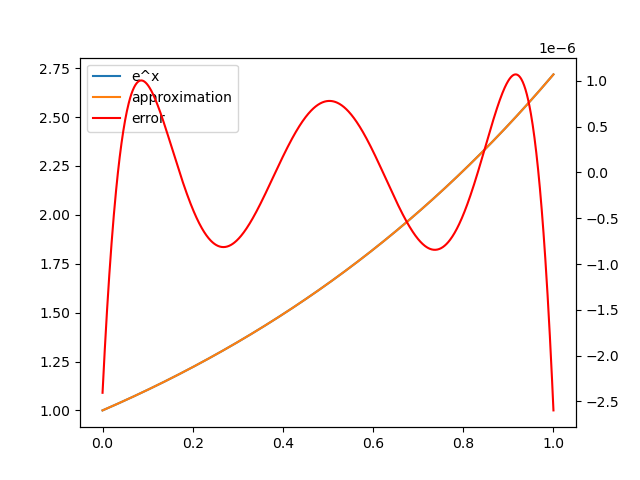
\includegraphics[width=0.8\textwidth]{../picture/Seventh_Week_1A.png}
    \caption{$n=5$,$\varphi(x)=x^{k}$}
    \label{pic:1}
\end{figure}

\subsection{对\ref{Q2}的解答}
Legendre多项式是定义在$[-1,1]$上以1为权函数的直化多项式,故需做变换$u=\frac{x+1}{2}$将其变换到区间$[0,1]$上。
令$g(x)=l(2x-1)$($l$为Legendre多项式),则$g(x)$为定义在$[0,1]$上的以1为权函数的直化多项式。类似于书上的推导,
我们有:
\begin{equation}
    a_j=\frac{\int_{0}^{1} g(x)f(x)dx}{\int_{0}^{1} g(x)^2dx}=(2j+1)\int_{0}^{1} g(x)f(x)dx,j=0,1,\cdots,n
\end{equation}
使用Python实现,代码见\cref{code2}。
如\cref{pic:2}。
\begin{figure}[H]
    \centering
    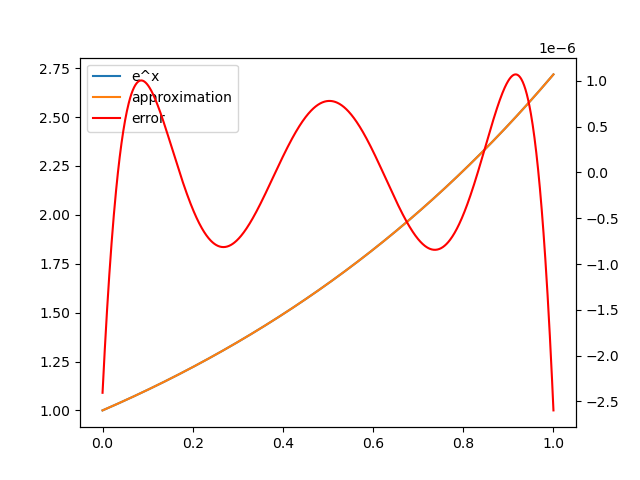
\includegraphics[width=0.8\textwidth]{../picture/Seventh_Week_1B.png}
    \caption{$n=5$,$\varphi(x)$为$k$次Legendre多项式}
    \label{pic:2}
\end{figure}

\subsection{对\ref{Q3}的解答}
方法同\ref{Q1},使用Python实现,代码见\cref{code3}。
如\cref{pic:3}。
\begin{figure}[H]
    \centering
    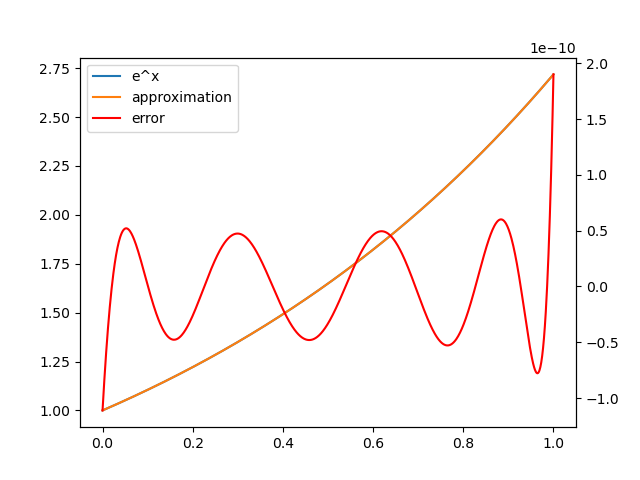
\includegraphics[width=0.8\textwidth]{../picture/Seventh_Week_1C.png}
    \caption{$n=10$,$\varphi(x)=x^{k}$}
    \label{pic:3}
\end{figure}

\subsection{对\ref{Q4}的解答}
方法同\ref{Q2},使用Python实现,代码见\cref{code4}。
如\cref{pic:4}。
\begin{figure}[H]
    \centering
    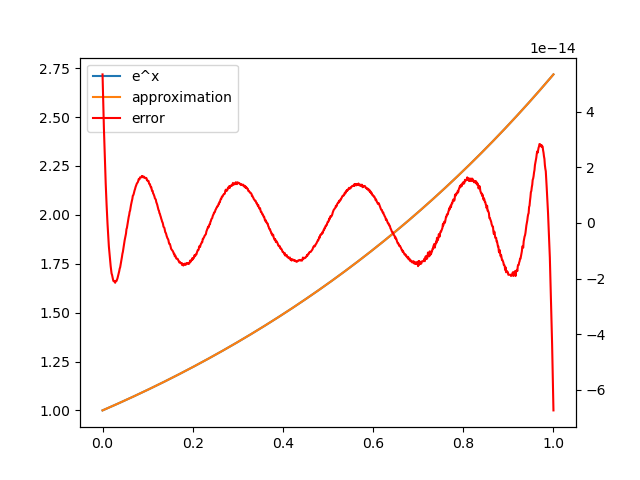
\includegraphics[width=0.8\textwidth]{../picture/Seventh_Week_1D.png}
    \caption{$n=10$,$\varphi(x)$为$k$次Legendre多项式}
    \label{pic:4}
\end{figure}

\subsection{对\ref{Q5}的解答}
我们使用Cooley-Tukey FFT算法实现了FFT(见\cref{code5}),并使用FFT对正弦信号进行压缩,保留大于100的频率成分,截断其他成分(见\cref{code5})。\\
如\cref{pic:5}。
\begin{figure}[H]
    \centering
    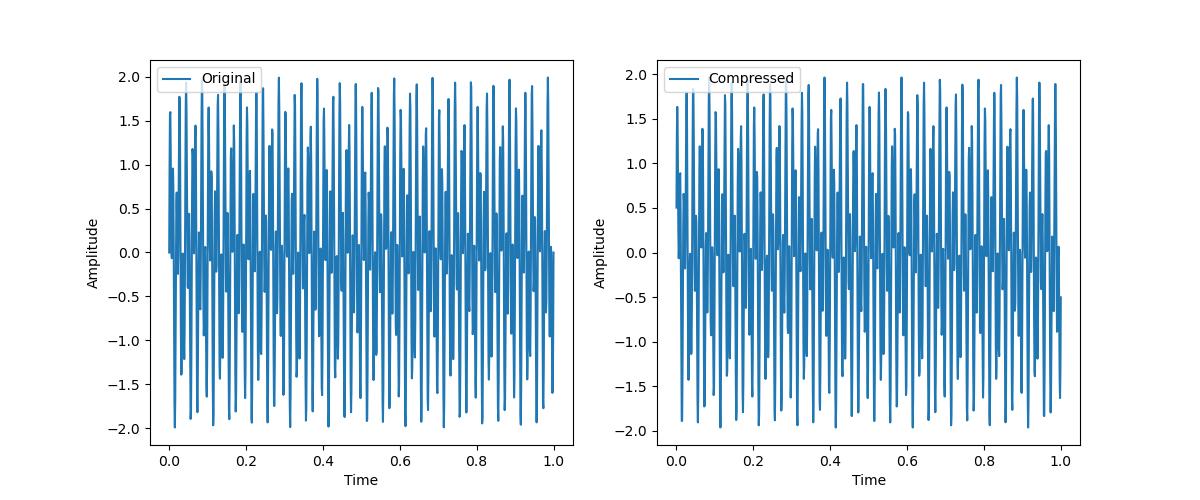
\includegraphics[width=0.8\textwidth]{../picture/Seventh_Week_2.png}
    \caption{压缩正弦信号}
    \label{pic:5}
\end{figure}

\section{结果分析}
\subsection{对\ref{Q1},\ref{Q2},\ref{Q3},\ref{Q4}的分析}
程序计算出相应多项式系数的运行时间如下:(我们取运行50次的时间平均值)
\begin{center}
\begin{tabular}{|c|c|c|}
\hline
Run time(s)& $\varphi(x)=x^{k}$ & $\varphi(x)$为$k$次Legendre多项式 \\
\hline
$n=5$& 0.11888313293457031 & 0.12630319595336914\\
\hline
$n=10$&0.12168169021606445 & 0.14491581916809082\\
\hline
\end{tabular}
\end{center}
可以看到时间差距并不大,于是我们取n=100、1000,再做观察:
\begin{center}
\begin{tabular}{|c|c|c|}
\hline
Run time(s)& $\varphi(x)=x^{k}$ & $\varphi(x)$为$k$次Legendre多项式 \\
\hline
$n=100$& 0.13881516456604004 & 0.35213565826416016\\
\hline
$n=1000$&22.1142737865448 & 60+\\
\hline
\end{tabular}
\end{center}
可以看到n增大后,由于计算Legendre多项式的负担,使用Legendre多项式作为基函数
反而用时更长,且估计可知Legendre多项式系数会发生上溢。\\
\indent 但观察图片可知,使用Legendre多项式作为基函数的误差随着n的增大会以数量级小于
使用$x^k$作为基函数的误差,这和我们理论分析的结论是一致的:计算含Hilbert矩阵
的线性方程组时出现的舍入误差会产生干扰。

\section{附录:程序代码}
\begin{lstlisting}[language=Python,caption={Seventh Week 1A.py},label={code1}]
import numpy as np
from matplotlib import pyplot as plt
from scipy.integrate import quad
from scipy.linalg import hilbert
import time

def f(x, k):
    return x**k * np.exp(x)

def integral(k,f): 
    result, error = quad(f, 0, 1, args=(k,))
    return result

def approx(x, a):
    return sum(a[i] * x**i for i in range(len(a)))
start=time.time()
n=5
b=np.array([integral(i,f=f) for i in range(n+1)])
A=hilbert(n+1)
X=np.linalg.solve(A,b)
fig,ax1=plt.subplots()
x = np.linspace(0, 1, 1000)
y = np.e**x
y_approx = approx(x, X)
end=time.time()
print("run time:",end-start)
line1,=ax1.plot(x, y, label='e^x')
line2,=ax1.plot(x, y_approx, label='approximation')
ax2=ax1.twinx()
line3,=ax2.plot(x,y_approx-y,label='error',color='r')
lines = [line1, line2, line3]
labels = [l.get_label() for l in lines]
ax1.legend(lines, labels,loc='best')
plt.show()
\end{lstlisting}

\begin{lstlisting}[language=Python,caption={Seventh Week 1B.py},label={code2}]
import numpy as np
from matplotlib import pyplot as plt
from scipy.integrate import quad
from scipy.special import legendre
import time

def f(x, k):
    return legendre(k)(2*x-1) * np.exp(x)

def integral(k, func):
    result, error = quad(func, 0, 1, args=(k,))
    return result

def approx(x, a):
    return sum(a[i] * legendre(i)(2*x-1) for i in range(len(a)))

start=time.time()
n = 5
coefficient = np.array([(2*i+1)*integral(i, f) for i in range(n+1)])

fig, ax1 = plt.subplots()
x = np.linspace(0, 1, 1000)
y = np.e**x
y_approx = approx(x, coefficient)
end=time.time()
print("run time:",end-start)
line1, = ax1.plot(x, y, label='e^x')
line2, = ax1.plot(x, y_approx, label='approximation')
ax2 = ax1.twinx()
line3, = ax2.plot(x, y_approx-y, label='error', color='r')
lines = [line1, line2, line3]
labels = [l.get_label() for l in lines]
ax1.legend(lines, labels, loc='best')
plt.show()       
\end{lstlisting}

\begin{lstlisting}[language=Python,caption={Seventh Week 1C.py},,label={code3}]
import numpy as np
from matplotlib import pyplot as plt
from scipy.integrate import quad
from scipy.linalg import hilbert
import time

def f(x, k):
    return x**k * np.exp(x)

def integral(k,f): 
    result, error = quad(f, 0, 1, args=(k,))
    return result

def approx(x, a):
    return sum(a[i] * x**i for i in range(len(a)))
start=time.time()
n=10
b=np.array([integral(i,f=f) for i in range(n+1)])
A=hilbert(n+1)
X=np.linalg.solve(A,b)
fig,ax1=plt.subplots()
x = np.linspace(0, 1, 1000)
y = np.e**x
y_approx = approx(x, X)
end=time.time()
print("run time:",end-start)
line1,=ax1.plot(x, y, label='e^x')
line2,=ax1.plot(x, y_approx, label='approximation')
ax2=ax1.twinx()
line3,=ax2.plot(x,y_approx-y,label='error',color='r')
lines = [line1, line2, line3]
labels = [l.get_label() for l in lines]
ax1.legend(lines, labels,loc='best')
plt.show()
\end{lstlisting}

\begin{lstlisting}[language=Python,caption={Seventh Week 1D.py},label={code4}]
import numpy as np
from matplotlib import pyplot as plt
from scipy.integrate import quad
from scipy.special import legendre
import time

def f(x, k):
    return legendre(k)(2*x-1) * np.exp(x)

def integral(k, func):
    result, error = quad(func, 0, 1, args=(k,))
    return result

def approx(x, a):
    return sum(a[i] * legendre(i)(2*x-1) for i in range(len(a)))

start=time.time()
n = 10
coefficient = np.array([(2*i+1)*integral(i, f) for i in range(n+1)])

fig, ax1 = plt.subplots()
x = np.linspace(0, 1, 1000)
y = np.e**x
y_approx = approx(x, coefficient)
end=time.time()
print("run time:",end-start)
line1, = ax1.plot(x, y, label='e^x')
line2, = ax1.plot(x, y_approx, label='approximation')
ax2 = ax1.twinx()
line3, = ax2.plot(x, y_approx-y, label='error', color='r')
lines = [line1, line2, line3]
labels = [l.get_label() for l in lines]
ax1.legend(lines, labels, loc='best')
plt.show()      
\end{lstlisting}

\begin{lstlisting}[language=Python,caption={Seventh Week 2.py},label={code5}]
import numpy as np
import matplotlib.pyplot as plt

def fft(x):
    N = len(x)
    if N == 1:
        return x
    even = fft(x[0::2])
    odd = fft(x[1::2])
    freq = np.zeros(N, dtype=complex)
    for k in range(N//2):
        t = np.exp(-2j * np.pi * k / N) * odd[k]
        freq[k] = even[k] + t
        freq[k + N//2] = even[k] - t
    return freq

def ifft(x):
    N = len(x)
    if N == 1:
        return x
    even = ifft(x[0::2])
    odd = ifft(x[1::2])
    time = np.zeros(N, dtype=complex)
    for k in range(N//2):
        t = np.exp(2j * np.pi * k / N) * odd[k]
        time[k] = even[k] + t
        time[k + N//2] = even[k] - t
    return time

N = 1024
t = np.linspace(0, 1, N)
x = np.sin(2 * np.pi * 50 * t) + np.sin(2 * np.pi * 120 * t)
X = fft(x)

X_mag = np.abs(X)
X_mag[X_mag < 100] = 0
X2 = X_mag * np.exp(1j * np.angle(X))

x2 = np.real(ifft(X2)/N)

plt.figure(figsize=(12, 5))
plt.subplot(121)
plt.plot(t, x, label='Original')
plt.xlabel('Time')
plt.ylabel('Amplitude')
plt.legend()
plt.subplot(122)
plt.plot(t, x2, label='Compressed')
plt.xlabel('Time')
plt.ylabel('Amplitude')
plt.legend()
plt.show()
\end{lstlisting}
\end{document}